\documentclass[tikz,border=2pt]{standalone}
\usepackage{amsmath}
\usepackage{pgfplots}
\pgfplotsset{compat=1.18}

\begin{document}
% a_n = (-1)^n (1 + 1/n): bounded (all terms lie between -2 and 2) but not convergent.
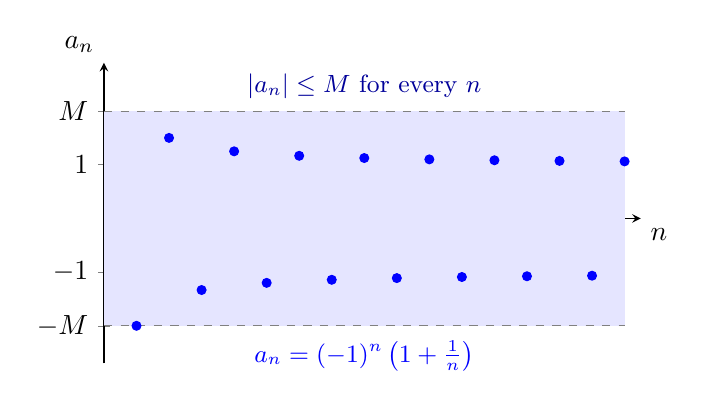
\begin{tikzpicture}
	\begin{axis}[
		axis lines=middle,
		xmin=0, xmax=16.5,
		ymin=-2.7, ymax=2.9,
		xtick={1,5,10,15}, ytick={-2,-1,1,2}, yticklabels={$-M$,$-1$,$1$,$M$},
		xlabel={$n$}, ylabel={$a_n$},
		xlabel style={below right}, ylabel style={above left},
		clip=false,
		width=8.4cm, height=5.4cm
		]
		\fill[blue!10] (axis cs:0,-2) rectangle (axis cs:16,2);
		\addplot[gray, dashed, domain=0:16] {2};
		\addplot[gray, dashed, domain=0:16] {-2};
		\addplot[only marks, mark=*, mark size=1.6pt, blue, samples at={1,...,16}] {(-1)^x*(1+1/x)};
		\node[blue!60!black, anchor=south, font=\small] at (axis cs:8,2.05) {$|a_n|\le M$ for every $n$};
		\node[blue, anchor=north, font=\small] at (axis cs:8,-2.1) {$a_n=(-1)^n\left(1+\tfrac1n\right)$};
	\end{axis}
\end{tikzpicture}
\end{document}
